\chapter{Implementation}
% This chapter should describe what was actually produced: the programs which were written, the hardware which was built or the theory which was developed. Any design strategies that looked ahead to the testing stage might profitably be referred to (the professional approach again).
% Descriptions of programs may include fragments of high-level code but large chunks of code are usually best left to appendices or omitted altogether. Analogous advice applies to circuit diagrams.
% Draw attention to the parts of the work which are not your own. The Implementation Chapter should include a section labelled ”Repository Overview”. The repository overview should be around one page in length and should describe the high-level structure of the source code found in your source code Repository. It should describe whether the code was written from scratch or if it built on an existing project or tutorial. Making effective use of powerful tools and pre-existing code is often laudable, and will count to your credit if properly reported.
% It should not be necessary to give a day-by-day account of the progress of the work but major milestones may sometimes be highlighted with advantage.

%  ~4,500 words

Could be split into \textit{preprocessing, parameter tuning, evaluation framework, software engineering techniques, repository overview}

Pipeline:
1) PREPARATION section:
precompute similarity matrices, functional connectivity matrices, a more convenient lookup table – with testing; design considerations for performance: 85hrs vs the smart matrix multiplication – give the maths!;
PCA of functional data;
UK Biobank IDs 
sorting subjects so that they are present in all modalities
removing subjects with invalid functional connectivity matrices
testing
2) graph SETUP:
similarity function development, 
specification parameters for functional, structural, euler index data
similarity function specification
3) graph TRANSFORM:
normalisation, edge computation based on similarity thresholds, internal structure of the population graph object with raw data in dictionaries; normalisation on demand
4) training SETUP: cross validation, stratification, creating final feature vectors on demand only
5) implementation of the NETWORKS: description of architecture: number and size of layers, other tunable parameters in practice and which hyperparameters will be experimented with
6) EVALUATION framework: describe the additional graph transformation stages which add noise to node features/edges.

% Tangent works better than correlation or partial correlation.


\subsection{Graph construction pipeline}
TODO update
\begin{figure}[!ht]
    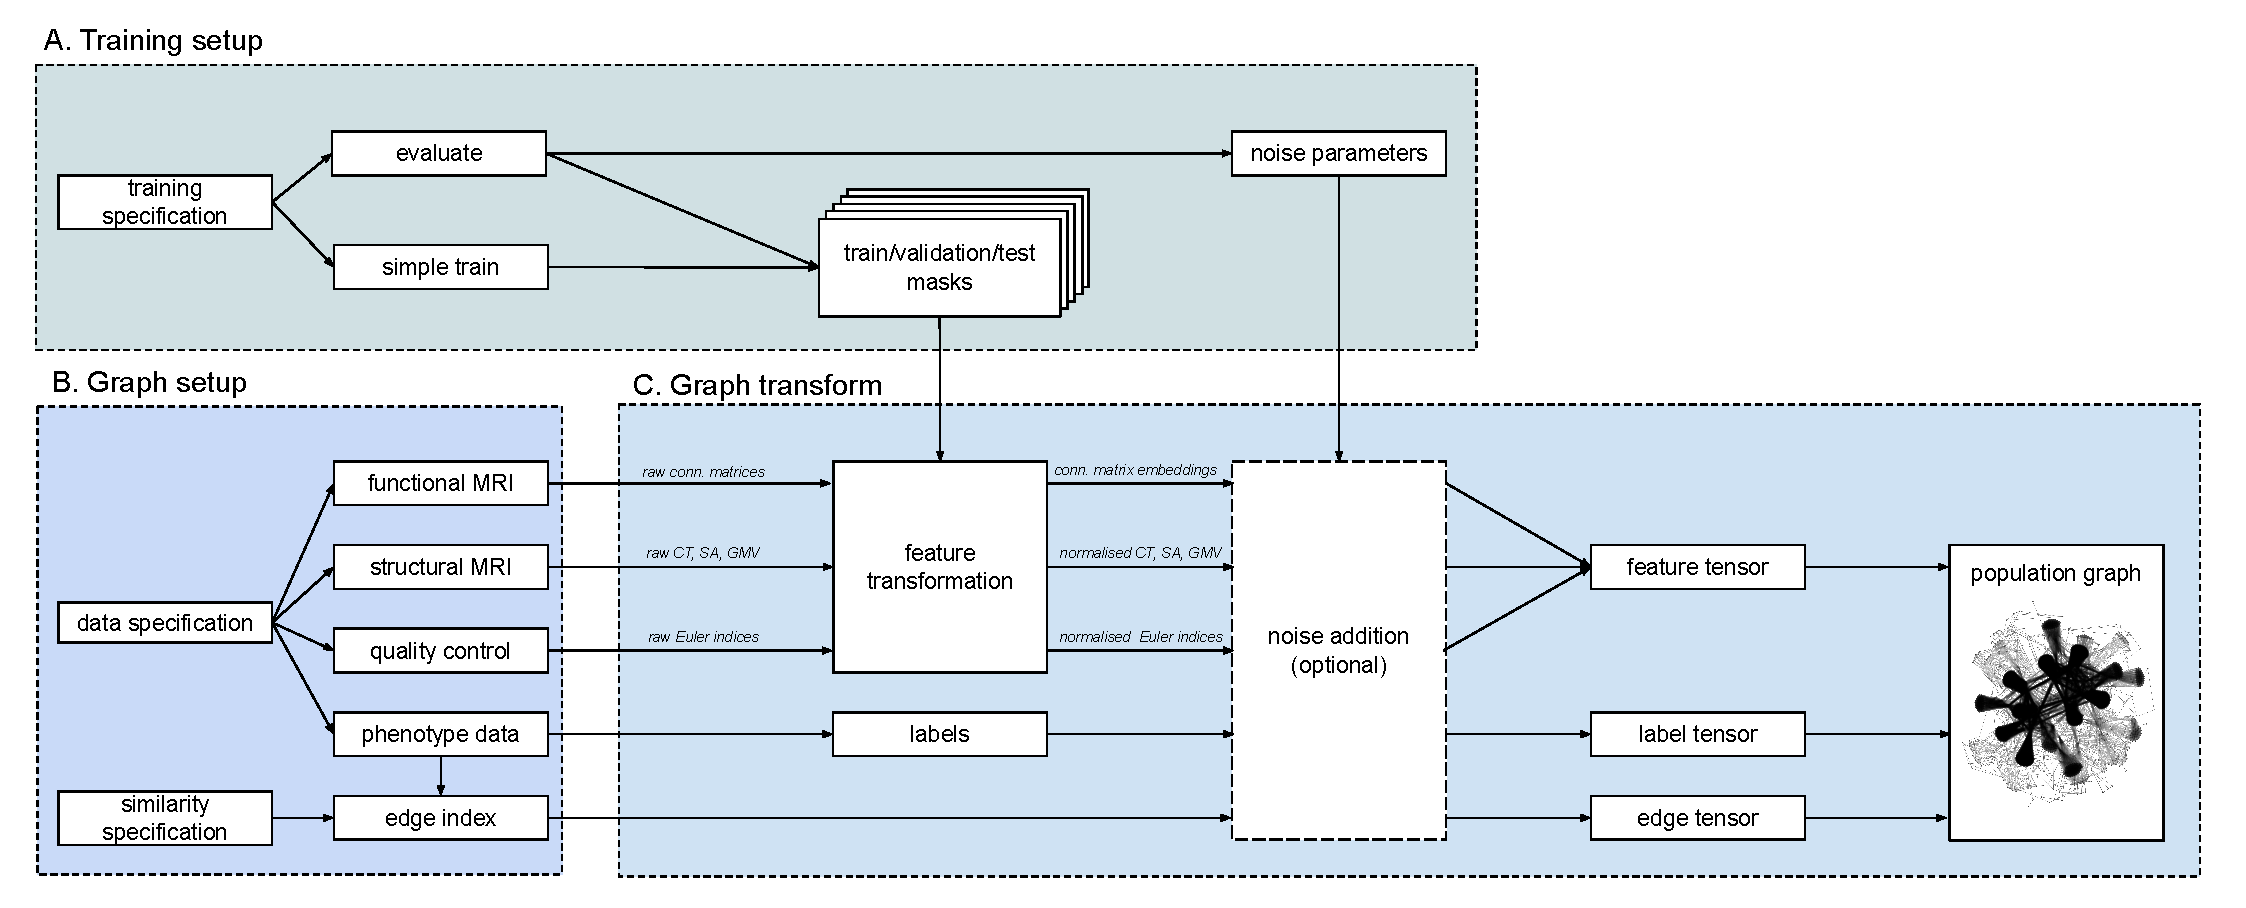
\includegraphics[width=\textwidth]{graphpipeline.pdf}
    \label{graphpipeline}
    \caption{Graph pipeline.}
\end{figure}


\section{Repository overview}
% TODO  The repository overview should be around one page in length and should describe the high-level structure of the source code found in your source code Repository; ... could be implemented as a table with folders/file names and the functionality implemented in those files

TODO rougly split into \textit{precompute} (with tests), \textit{preprocessing} (with tests?), \textit{similarity} (with tests), \textit{evaluation}, \textit{brainGAT, brainGCN}, ... 

